% Payload-Aware Two-Tier UAV Route Planning — Review I Presentation
% Compile with: pdflatex Review1_Presentation.tex  (run twice)

\documentclass[aspectratio=169,11pt]{beamer}

% ---------- Theme and colours ----------
\usetheme{Madrid}
\usecolortheme{default}
\definecolor{UniversityBlue}{RGB}{16,62,110}
\definecolor{AccentBlue}{RGB}{30,136,229}
\definecolor{LightBlue}{RGB}{232,242,252}
\definecolor{DarkGray}{RGB}{55,65,81}

\setbeamercolor{structure}{fg=UniversityBlue}
\setbeamercolor{palette primary}{bg=UniversityBlue,fg=white}
\setbeamercolor{palette secondary}{bg=AccentBlue,fg=white}
\setbeamercolor{frametitle}{bg=UniversityBlue,fg=white}
\setbeamercolor{block title}{bg=UniversityBlue,fg=white}
\setbeamercolor{block body}{bg=LightBlue,fg=black}
\setbeamercolor{alerted text}{fg=AccentBlue}

% ---------- Packages ----------
\usepackage[T1]{fontenc}
\usepackage[utf8]{inputenc}
\usepackage{lmodern}
\usepackage{graphicx}
\graphicspath{{../Phase 1 Report/diagrams/}{./}}
\usepackage{booktabs}
\usepackage{array}
\usepackage{tabularx}
\usepackage{tikz}
\usetikzlibrary{positioning}
\usepackage{amsmath}
\usepackage{listings}
\usepackage{xcolor}
\usepackage{colortbl}
\usepackage{microtype}
\usepackage{hyperref}

\newcolumntype{Y}{>{\raggedright\arraybackslash}X}

% ---------- General settings ----------
\setbeamertemplate{navigation symbols}{}
\setbeamertemplate{caption}[numbered]
\setbeamertemplate{itemize item}{\color{AccentBlue}$\blacktriangleright$}
\setbeamertemplate{itemize subitem}{\color{UniversityBlue}$\bullet$}
\setbeamersize{text margin left=0.7cm,text margin right=0.7cm}

% Footer: project title, institution and slide number
\setbeamertemplate{footline}{%
  \leavevmode%
  \hbox{%
    \begin{beamercolorbox}[wd=.42\paperwidth,ht=2.7ex,dp=1.1ex,leftskip=.6em]{author in head/foot}%
      \insertshorttitle
    \end{beamercolorbox}%
    \begin{beamercolorbox}[wd=.46\paperwidth,ht=2.7ex,dp=1.1ex,center]{date in head/foot}%
      Department of Computer Science and Engineering
    \end{beamercolorbox}%
    \begin{beamercolorbox}[wd=.12\paperwidth,ht=2.7ex,dp=1.1ex,center]{page number in head/foot}%
      \insertframenumber/\inserttotalframenumber
    \end{beamercolorbox}%
  }%
  \vskip0pt%
}

% ---------- Editable project details ----------
\title[Payload-Aware Two-Tier UAV Route Planning]{%
  Payload-Aware Two-Tier UAV Route Planning\\for Last-Mile Delivery}
\subtitle{Review Report -- I}
\author[Thirumurugan $\cdot$ Shrika $\cdot$ Meghna]{%
  \texorpdfstring{%
    Thirumurugan RA \hfill (3122235001149)\\[1mm]
    Meghna Manimaran \hfill (3122235001079)\\[1mm]
    Shrika SP Thota \hfill (3122235001125)%
  }{Thirumurugan RA, Meghna Manimaran, Shrika SP Thota}%
}
\institute[SSN College of Engineering]{%
  Guided by: Sujaudeen N, Assistant Professor\\[2mm]
  Department of Computer Science and Engineering\\
  Sri Sivasubramaniya Nadar College of Engineering%
}
\date{Academic Year 2026--2027}
\hypersetup{
  pdftitle={Payload-Aware Two-Tier UAV Route Planning for Last-Mile Delivery},
  pdfauthor={Thirumurugan RA, Meghna Manimaran, Shrika SP Thota}
}

\begin{document}

% ── 1. Title slide ──────────────────────────────────────────────────────────
\begin{frame}[plain]
  \titlepage
  \begin{tikzpicture}[remember picture,overlay]
    \node[anchor=north east,xshift=-0.4cm,yshift=-0.3cm]
      at (current page.north east)
      {
\includegraphics[width=1.5cm]{ssn-logo.png}};
  \end{tikzpicture}
\end{frame}

% ── 2. Outline ──────────────────────────────────────────────────────────────
\begin{frame}{Presentation Outline}
  \tableofcontents
\end{frame}

% ════════════════════════════════════════════════════════════════
\section{Introduction}
% ════════════════════════════════════════════════════════════════

% ── 3. Background and Motivation ────────────────────────────────────────────
\begin{frame}{Background and Motivation}
  \begin{columns}[T,onlytextwidth]
    \column{0.58\textwidth}
      \begin{itemize}
        \item Urban last-mile delivery is rapidly shifting to autonomous UAV
              platforms for speed, flexibility, and scalability.
        \item Existing routing systems treat all deliveries
              \textbf{identically} — a fragile medical device and a robust
              parcel travel the \emph{same} route.
        \item Payload-specific risk, energy, and safety constraints are
              completely ignored by current approaches.
        \item Payload metadata (urgency, fragility, payload weight)
              encodes routing priorities, but no system exploits this
              information at query time.
      \end{itemize}
    \column{0.38\textwidth}
      \begin{block}{Core Motivation}
        Fragmented UAV routing pipelines cannot adapt to cargo-specific
        constraints in real time.  A two-tier architecture that bridges
        payload semantics to route selection addresses this gap.
      \end{block}
  \end{columns}
\end{frame}

% ── 4. Problem Statement ────────────────────────────────────────────────────
\begin{frame}{Problem Statement}
  \begin{alertblock}{Problem}
    Existing UAV routing systems apply \textbf{static, cargo-agnostic
    objective weights}, resulting in \textbf{suboptimal or unsafe routes}
    for payloads with differing fragility, urgency, and payload weight.
  \end{alertblock}
  \vspace{0.35cm}
  \begin{itemize}
    \item Given payload metadata $(U,\,F,\,T)\in\{1\ldots5\}^3$ and a
          weighted airspace graph $G=(V,E,W)$, find route $\pi^*$ from
          source $s$ to destination $d$ that simultaneously minimises
          risk, distance, and energy.
    \item Single-objective routing cannot model conflicting objectives.
    \item No system dynamically translates cargo semantics into routing
          objective weights.
    \item Constraints: feasible path, energy $\leq$ battery capacity,
          risk $\leq$ threshold, selection latency within onboard budget.
  \end{itemize}
\end{frame}

% ── 5. Objectives ───────────────────────────────────────────────────────────
\begin{frame}{Project Objectives}
  \begin{enumerate}
    \item To build a \textbf{multi-objective A* engine (Tier~1)} that
          constructs a Pareto-efficient route set over a weighted airspace
          graph, balancing risk, distance, and energy objectives.
    \item To design an \textbf{algebraic bridge} that translates payload
          metadata tags (urgency~$U$, fragility~$F$, weight~$W$) into
          normalised routing objective weights in real time.
    \item To implement a \textbf{Tier~2 payload-driven selector} that scores
          each Pareto route using derived weights and returns the
          utility-maximising route~$\pi^*$.
    \item To evaluate the two-tier pipeline using \textbf{simulation
          benchmarks} against single-objective Dijkstra and A* baselines.
    \item To validate the system on \textbf{real drone hardware}
          (Raspberry Pi~5 + Pixhawk) through outdoor flight tests.
  \end{enumerate}
\end{frame}

% ── 6. Scope ────────────────────────────────────────────────────────────────
\begin{frame}{Scope and Expected Outcomes}
  \begin{columns}[T,onlytextwidth]
    \column{0.48\textwidth}
      \begin{block}{Included}
        \begin{itemize}
          \item Payload-aware UAV route selection for single-drone delivery
          \item Two-tier pipeline: Pareto front construction + utility
                selection
          \item Software simulation on OpenStreetMap urban graphs
                (Chennai area)
          \item RPi~5 + Pixhawk hardware integration and outdoor flight
                tests
          \item Benchmark against Dijkstra and single-objective A*
        \end{itemize}
      \end{block}
    \column{0.48\textwidth}
      \begin{block}{Excluded / Constraints}
        \begin{itemize}
          \item Multi-drone fleet management and coordination
          \item Real-time dynamic obstacle avoidance
          \item Commercial deployment and regulatory compliance
          \item Weather-based in-flight re-routing
          \item Deep-learning-based risk estimation
        \end{itemize}
      \end{block}
  \end{columns}
\end{frame}

% ════════════════════════════════════════════════════════════════
\section{Literature Review}
% ════════════════════════════════════════════════════════════════

% ── 7. Literature table ─────────────────────────────────────────────────────
\begin{frame}{Literature Review}
  \scriptsize
  \begin{tabularx}{\textwidth}{%
      >{\raggedright\arraybackslash}p{2.5cm}
      >{\raggedright\arraybackslash}p{2.9cm}
      >{\raggedright\arraybackslash}p{3.0cm}
      >{\raggedright\arraybackslash}X}
    \toprule
    \textbf{Author / Year} & \textbf{Method} &
    \textbf{Key Contribution} & \textbf{Limitation / Research Gap}\\
    \midrule
    Chokkalingam \& Ganesan (2026) &
      Entropy-based Pareto front &
      Maximises route diversity via information entropy; robust across
      urban environments &
      No payload awareness; weights are static across all cargo types\\
    \addlinespace
    Datsko et al.\ (2024) &
      Geometric Pareto spread &
      Uniform spread reduces clustering in the objective space &
      Fixed objective weights — cannot adapt dynamically to cargo
      semantics\\
    \addlinespace
    Ntakolia et al.\ (2023) &
      Crowding-distance Pareto selection &
      Well-distributed, representative Pareto solutions via crowding
      distance &
      No semantic metadata integration at query time; selection is
      cargo-agnostic\\
    \bottomrule
  \end{tabularx}
\end{frame}

% ── 8. Gap and novelty ──────────────────────────────────────────────────────
\begin{frame}{Research Gap and Proposed Contribution}
  \begin{columns}[T,onlytextwidth]
    \column{0.47\textwidth}
      \begin{block}{Identified Gaps}
        \begin{itemize}
          \item No unified end-to-end pipeline for payload-aware UAV
                routing exists
          \item All cargo types receive identical routing weights
          \item No work maps fragility / urgency / payload weight
                to Pareto utility scores
          \item Most approaches are simulation-only; none validate on real
                drone hardware
        \end{itemize}
      \end{block}
    \column{0.49\textwidth}
      \begin{block}{Proposed Contribution}
        \begin{itemize}
          \item Two-tier pipeline: Tier~1 Pareto front + Tier~2
                payload-aware selector
          \item Algebraic bridge: cargo metadata
                $\rightarrow$ normalised routing weights
          \item Utility-maximising selection:
                $\pi^* = \arg\max_{p_i\in P^*}\!\operatorname{score}(p_i)$
          \item Full hardware validation on RPi~5 + Pixhawk drone
        \end{itemize}
      \end{block}
  \end{columns}
\end{frame}

% ════════════════════════════════════════════════════════════════
\section{System Design}
% ════════════════════════════════════════════════════════════════

% ── 9. Existing vs Proposed ─────────────────────────────────────────────────
\begin{frame}{Existing System vs.\ Proposed System}
  \small
  \begin{tabularx}{\textwidth}{>{\bfseries\raggedright\arraybackslash}p{2.9cm}YY}
    \toprule
    Criterion & Existing Routing Systems & Proposed Two-Tier System\\
    \midrule
    Routing approach &
      Single-objective (distance or energy only) &
      Multi-objective A* — risk, distance, energy simultaneously\\
    Payload handling &
      Cargo-agnostic; all parcels treated identically &
      Payload metadata $(U,F,T)$ drives objective weights dynamically\\
    Route selection &
      Single greedy optimal path &
      Pareto front + utility-based selection\\
    Adaptability &
      Fixed weights across all deliveries &
      Per-request weight derivation from cargo tags\\
    Hardware validation &
      Simulation only &
      RPi~5 + Pixhawk outdoor flight tests\\
    \bottomrule
  \end{tabularx}
\end{frame}

% ── 10. Architecture ────────────────────────────────────────────────────────
\begin{frame}{Proposed System Architecture}
  \centering
  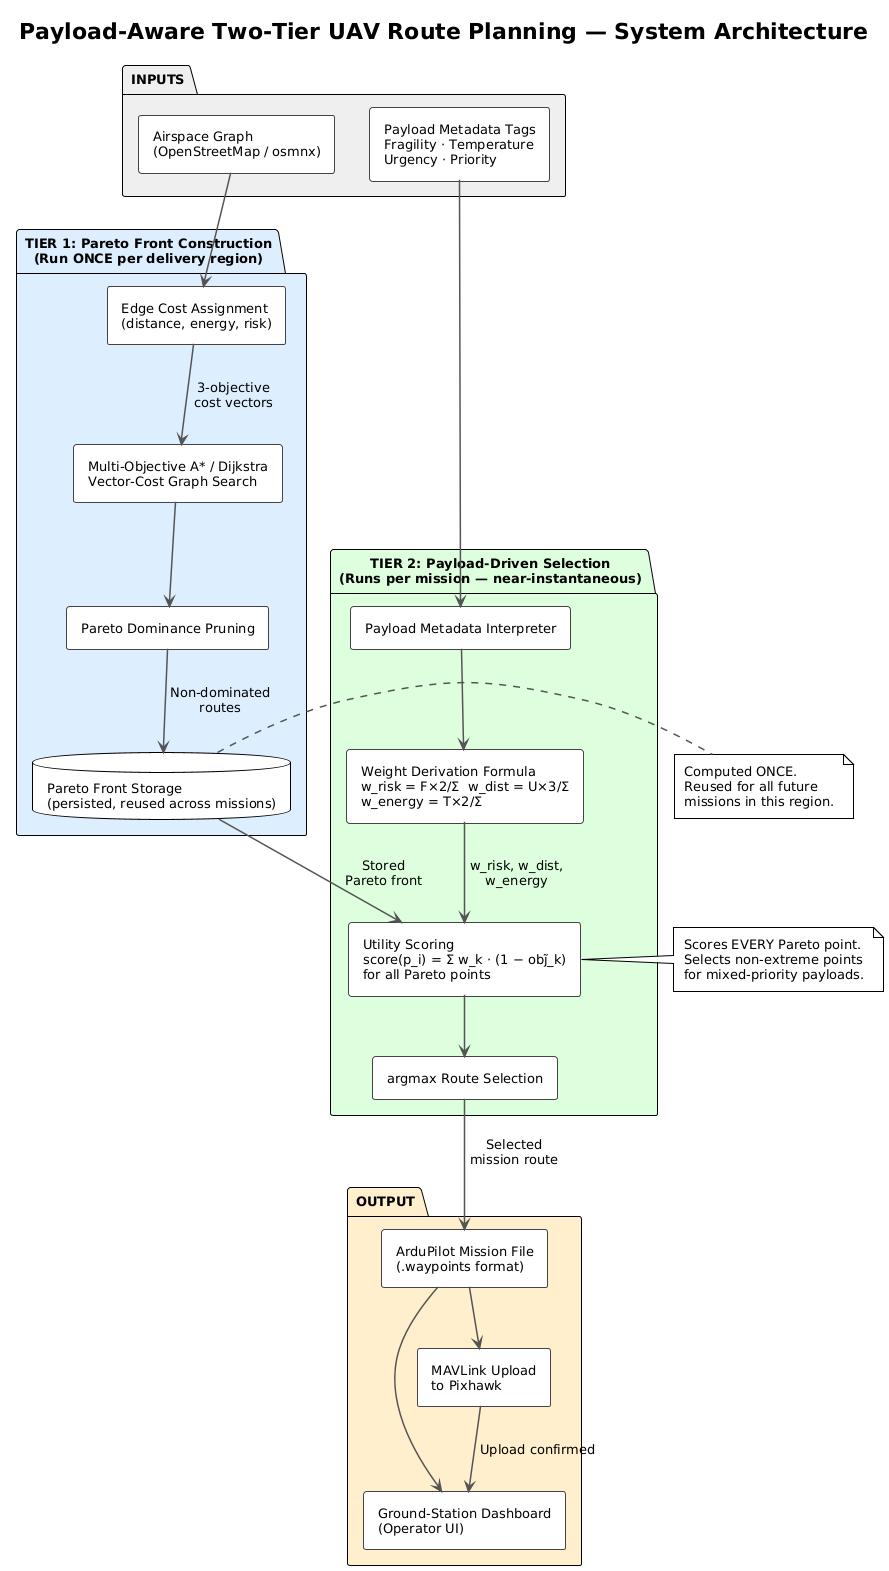
\includegraphics[width=0.88\textwidth,height=0.68\textheight,
                   keepaspectratio]{arch.png}
\end{frame}

% ── 11. Modules ─────────────────────────────────────────────────────────────
\begin{frame}{System Modules}
  \begin{enumerate}
    \item \textbf{M1 -- Data \& Input Management:}
          Receives delivery request, parses payload metadata $(U,F,T)$,
          validates inputs, and initialises the airspace graph using
          OpenStreetMap / OSMnx.

    \item \textbf{M2 -- Core Processing (Tier~1 A*):}
          Executes multi-objective A* search with 3-objective cost vectors
          $\mathbf{c}(e)=(\rho_e,\,d_e,\,\varepsilon_e)$, applies Pareto
          dominance pruning, and returns the Pareto front $P^*$.

    \item \textbf{M3 -- Payload Selector (Tier~2):}
          Applies the algebraic bridge to derive
          $w_\text{risk},w_\text{dist},w_\text{energy}$; min-max normalises
          Pareto objectives; computes utility scores; returns $\pi^*$.

    \item \textbf{M4 -- UI, Hardware \& Evaluation:}
          Provides operator dashboard (Flask / ROS~2), interfaces with
          RPi~5 + Pixhawk via MAVLink, and logs route metrics for
          benchmarking.
  \end{enumerate}
\end{frame}

% ── 12. Methodology ─────────────────────────────────────────────────────────
\begin{frame}{Methodology / Workflow}
  \begin{columns}[T,onlytextwidth]
    \column{0.62\textwidth}
      \begin{enumerate}
        \item Literature review and problem formulation
        \item Airspace graph construction (OpenStreetMap + OSMnx)
        \item Multi-objective A* engine implementation (Tier~1)
        \item Algebraic bridge and Pareto selector (Tier~2)
        \item Software simulation and benchmarking vs.\ baselines
        \item Hardware integration (RPi~5 + Pixhawk) and outdoor
              flight validation
      \end{enumerate}
    \column{0.34\textwidth}
      \begin{block}{Evaluation Metrics}
        \begin{itemize}
          \item Route risk score $\rho$
          \item Route distance (km)
          \item Energy consumption (Wh)
          \item Utility score vs.\ baseline
          \item Onboard latency (ms)
        \end{itemize}
      \end{block}
  \end{columns}
\end{frame}

% ── 13. Algorithm ───────────────────────────────────────────────────────────
\begin{frame}{Core Algorithm: Payload-Aware Two-Tier Route Planning}
  \begin{block}{Algorithm Summary}
    \begin{enumerate}
      \item \textbf{Input:} Graph $G=(V,E,W)$, payload tags $(U,F,T)$,
            source $s$, destination $d$.
      \item \textbf{Weight derivation (Algebraic Bridge):}\\
            $r_\text{raw}=F{\times}2$,\;
            $d_\text{raw}=U{\times}3$,\;
            $e_\text{raw}=T{\times}2$;\;
            normalise $\Rightarrow w_\text{risk},\,w_\text{dist},\,w_\text{energy}$.
      \item \textbf{Tier~1 --- Pareto search:} Run multi-objective A*;
            accumulate cost vectors; prune dominated paths; return front
            $P^*$.
      \item \textbf{Tier~2 --- Scoring:} For each $p_i\in P^*$,
            \[
              \operatorname{score}(p_i)=
                w_d(1-\tilde{d}_i)+w_\varepsilon(1-\tilde{\varepsilon}_i)
                +w_\rho(1-\tilde{\rho}_i)
            \]
      \item \textbf{Output:}
            $\pi^*=\arg\max_{p_i\in P^*}\operatorname{score}(p_i)$;
            generate ArduPilot mission file; upload via MAVLink.
    \end{enumerate}
  \end{block}
\end{frame}

% ── 14. Technology stack ────────────────────────────────────────────────────
\begin{frame}{Technology Stack and Resources}
  \small
  \begin{tabularx}{\textwidth}{>{\bfseries\raggedright\arraybackslash}p{3.1cm}Y}
    \toprule
    Category & Selected Technology / Resource\\
    \midrule
    Programming language  & Python 3.11\\
    Frameworks \& libraries & ROS~2 (Humble), NetworkX, OSMnx, Flask,
                              NumPy, SciPy\\
    Communication protocol & MAVLink / ArduPilot \texttt{.waypoints}
                             mission format\\
    Map / dataset          & OpenStreetMap airspace graph
                             (Chennai urban area)\\
    Development tools      & Git, VS Code, QGIS, Mission Planner,
                             SITL simulator, Docker\\
    Hardware               & Raspberry Pi~5 (quad-core 2.4\,GHz, 8\,GB),
                             Pixhawk~6C, GPS module, ESC + motors\\
    \bottomrule
  \end{tabularx}
\end{frame}

% ════════════════════════════════════════════════════════════════
\section{Implementation and Results}
% ════════════════════════════════════════════════════════════════

% ── 15. Implementation status ───────────────────────────────────────────────
\begin{frame}{Implementation Status}
  \small
  \begin{tabularx}{\textwidth}{Y>{\centering\arraybackslash}p{2.5cm}Y}
    \toprule
    \textbf{Component} & \textbf{Status} & \textbf{Evidence / Remarks}\\
    \midrule
    Literature review \& problem formulation &
      Completed & 3 papers surveyed; gap documented\\
    System design \& architecture &
      Completed & Two-tier architecture defined and diagrams produced\\
    Airspace graph construction &
      Completed & OSMnx graph over Chennai urban area loaded\\
    Tier~1: Multi-Objective A* engine &
      In Progress & Core A* with 3-objective cost vectors implemented\\
    Tier~2: Payload-driven selector &
      Planned & Algebraic bridge designed; coding next sprint\\
    Hardware integration (RPi~5 + Pixhawk) &
      Planned & Hardware procured; assembly and SITL setup pending\\
    \bottomrule
  \end{tabularx}
\end{frame}

% ── 16. Prototype diagrams ──────────────────────────────────────────────────
\begin{frame}{Prototype / Implementation Diagrams}
  \begin{columns}[T,onlytextwidth]
    \column{0.48\textwidth}
      \centering
      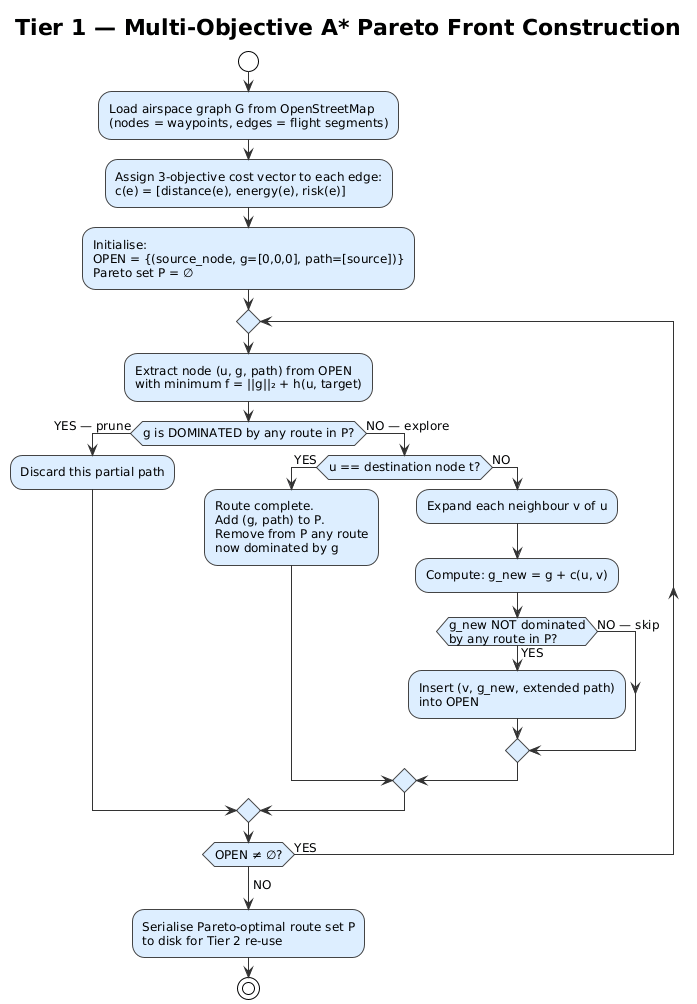
\includegraphics[width=\linewidth,height=4.1cm,keepaspectratio]{tier1.png}

      \small Tier~1: Multi-Objective A* Pareto Front Construction
    \column{0.48\textwidth}
      \centering
      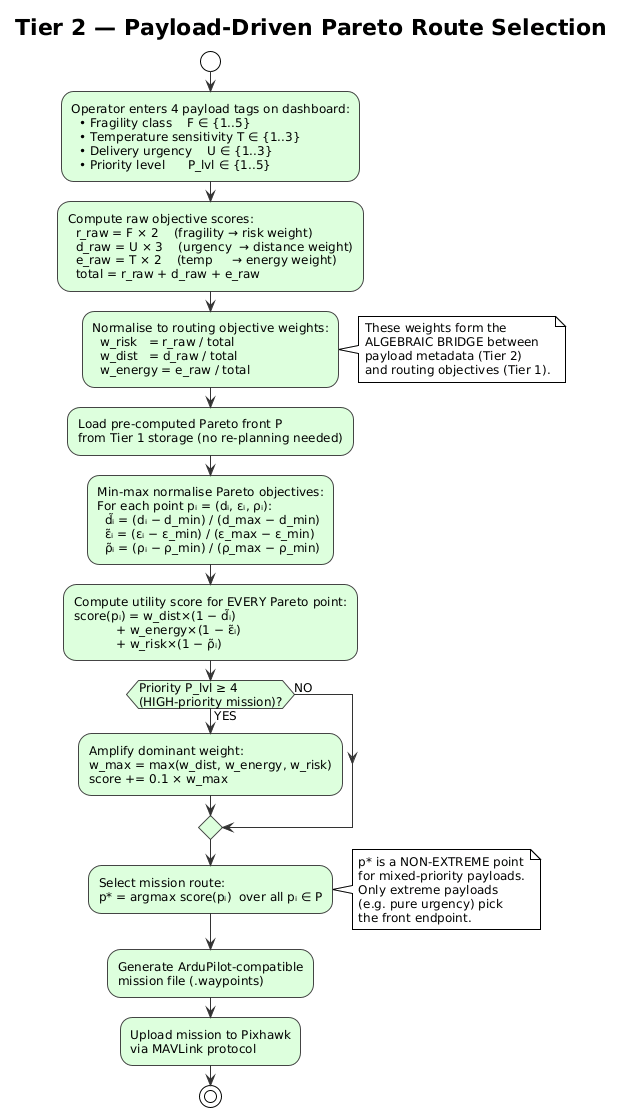
\includegraphics[width=\linewidth,height=4.1cm,keepaspectratio]{tier2.png}

      \small Tier~2: Payload-Driven Pareto Route Selection
  \end{columns}
\end{frame}

% ── 17. Results ─────────────────────────────────────────────────────────────
\begin{frame}{Expected Results and Performance Targets}
  \begin{columns}[T,onlytextwidth]
    \column{0.53\textwidth}
      \begin{block}{Example: Fragile Medical Payload}
        Input: $F{=}5,\;U{=}4,\;T{=}3$\\[4pt]
        $r_\text{raw}=10,\;d_\text{raw}=12,\;e_\text{raw}=6$\\[2pt]
        $w_\text{risk}=0.357,\;w_\text{dist}=0.429,\;
         w_\text{energy}=0.214$\\[4pt]
        High-risk edges are \textbf{heavily penalised}.\\
        Expected: significantly safer route than shortest-path baseline.
      \end{block}
    \column{0.43\textwidth}
      \begin{block}{Performance Targets}
        \begin{itemize}
          \item Risk score: $\geq\!20\%$ reduction vs.\ Dijkstra baseline
          \item Pareto front size: 5--15 non-dominated routes
          \item Tier~2 selection latency: $<\!50$\,ms on RPi~5
          \item Energy overhead: $\leq\!10\%$ above shortest-path route
          \item Hardware: successful outdoor delivery simulation flight
        \end{itemize}
      \end{block}
  \end{columns}
\end{frame}

% ── 18. Testing ─────────────────────────────────────────────────────────────
\begin{frame}{Testing and Validation Plan}
  \scriptsize
  \begin{tabularx}{\textwidth}{p{1.2cm} Y Y p{1.8cm}}
    \toprule
    \textbf{Test ID} & \textbf{Test Scenario} &
    \textbf{Expected Result} & \textbf{Status}\\
    \midrule
    TC-01 & Valid payload metadata $(U,F,T)$ input &
      Correct $w_\text{risk},w_\text{dist},w_\text{energy}$ derived &
      Planned\\
    TC-02 & Multi-objective A* on 100-node urban graph &
      Pareto front $P^*$ with zero dominated routes &
      Planned\\
    TC-03 & High fragility ($F{=}5$) vs.\ low fragility ($F{=}1$) &
      Significantly different route selected each time &
      Planned\\
    TC-04 & Disconnected graph (no feasible path) &
      Graceful error with clear user message &
      Planned\\
    TC-05 & RPi~5 MAVLink mission upload to Pixhawk &
      Drone accepts mission and executes flight &
      Planned\\
    \bottomrule
  \end{tabularx}
  \vspace{0.3cm}
  \begin{block}{Validation Method}
    Unit tests (pytest), simulation benchmarking against Dijkstra and
    single-objective A*, and outdoor UAV flight tests with recorded
    telemetry logs.
  \end{block}
\end{frame}

% ════════════════════════════════════════════════════════════════
\section{Project Management}
% ════════════════════════════════════════════════════════════════

% ── 19. Timeline ────────────────────────────────────────────────────────────
\begin{frame}{Project Timeline (Aug\,2026 -- Mar\,2027)}
  \scriptsize
  \begin{tabularx}{\textwidth}{Y*{8}{>{\centering\arraybackslash}p{0.66cm}}}
    \toprule
    \textbf{Activity} &
    \textbf{Aug} & \textbf{Sep} & \textbf{Oct} & \textbf{Nov} &
    \textbf{Dec} & \textbf{Jan} & \textbf{Feb} & \textbf{Mar}\\
    \midrule
    Literature survey \& formulation &
      \cellcolor{AccentBlue!35} & \cellcolor{AccentBlue!35} &&&&&& \\
    System design \& architecture &&
      \cellcolor{AccentBlue!35} &&&&&&\\
    Tier~1: Multi-Objective A* &&&
      \cellcolor{AccentBlue!35} &&&&&\\
    Tier~2: Payload-Driven Selector &&&&
      \cellcolor{AccentBlue!35} &&&&\\
    Software simulation \& benchmarking &&&&&
      \cellcolor{AccentBlue!35} &&&\\
    Hardware integration (RPi~5) &&&&&&
      \cellcolor{AccentBlue!35} &&\\
    Outdoor flight tests &&&&&&&
      \cellcolor{AccentBlue!35} &\\
    Documentation \& report writing &&&&&&&
      \cellcolor{AccentBlue!35} & \cellcolor{AccentBlue!35}\\
    \bottomrule
  \end{tabularx}
  \vspace{0.3cm}
  \small
  \textcolor{UniversityBlue}{\textbf{Review I:}} August 2026\qquad
  \textcolor{UniversityBlue}{\textbf{Final Submission:}} March 2027
\end{frame}

% ── 20. Responsibilities ────────────────────────────────────────────────────
\begin{frame}{Team Responsibilities}
  \small
  \begin{tabularx}{\textwidth}{>{\bfseries\raggedright\arraybackslash}p{3.3cm}Y p{2.3cm}}
    \toprule
    Team Member & Responsibilities & Current Status\\
    \midrule
    Thirumurugan RA &
      System architecture design, Tier~1 multi-objective A* engine,
      airspace graph construction (OSMnx) &
      In progress\\
    Shrika SP Thota &
      Algebraic bridge design, Tier~2 payload selector implementation,
      documentation &
      In progress\\
    Meghna Manimaran &
      Hardware procurement, RPi~5 + Pixhawk integration, testing and
      flight evaluation &
      Planned\\
    \bottomrule
  \end{tabularx}
\end{frame}

% ════════════════════════════════════════════════════════════════
\section{Conclusion}
% ════════════════════════════════════════════════════════════════

% ── 21. Challenges ──────────────────────────────────────────────────────────
\begin{frame}{Challenges, Risks, and Mitigation}
  \small
  \begin{tabularx}{\textwidth}{Y Y Y}
    \toprule
    \textbf{Risk / Challenge} & \textbf{Possible Impact} &
    \textbf{Mitigation}\\
    \midrule
    Graph complexity (large OSM urban network) &
      Slow Pareto search &
      Spatial pruning, epsilon-dominance, landmark heuristics\\
    Hardware failure (RPi / Pixhawk) &
      Flight tests delayed &
      SITL simulator validation first; spare hardware budget\\
    Pareto front size too large &
      High memory and selection latency &
      Apply epsilon-pruning to limit front size\\
    MAVLink integration issues &
      Mission upload failures &
      Validate protocol on SITL before real drone flights\\
    \bottomrule
  \end{tabularx}
\end{frame}

% ── 22. Conclusion and Future Work ──────────────────────────────────────────
\begin{frame}{Conclusion and Future Work}
  \begin{block}{Conclusion}
    This project addresses the critical gap of cargo-agnostic UAV routing by
    proposing a two-tier payload-aware pipeline.  Tier~1 builds a
    Pareto-efficient route set via multi-objective A*; Tier~2 selects the
    optimal route using an algebraic bridge that maps fragility, urgency, and
    payload weight into routing objective weights.  System design is
    complete and Tier~1 implementation is underway.
  \end{block}
  \begin{block}{Future Work}
    \begin{itemize}
      \item Outdoor flight validation on a real RPi~5 + Pixhawk drone in a
            simulated urban delivery environment.
      \item Extend to multi-drone coordination with shared Pareto fronts.
      \item Incorporate real-time weather and dynamic obstacle data for
            in-flight re-routing.
    \end{itemize}
  \end{block}
\end{frame}

% ── 23. References ──────────────────────────────────────────────────────────
\begin{frame}[allowframebreaks]{References}
  \footnotesize
  \begin{thebibliography}{9}

    \bibitem{r1}
      Chokkalingam and Ganesan,
      ``Entropy-based Pareto front for UAV path planning,'' 2026.

    \bibitem{r2}
      Datsko et al.,
      ``Geometric spread for multi-objective UAV routing,'' 2024.

    \bibitem{r3}
      Ntakolia et al.,
      ``Crowding-distance Pareto selection for UAV paths,''
      \emph{Journal of Computer Science}, 2023.

    \bibitem{r4}
      G.\ Boeing,
      ``OSMnx: New methods for acquiring, constructing, analysing, and
      visualising complex street networks,''
      \emph{Computers, Environment and Urban Systems}, vol.~65,
      pp.~126--139, 2017.
      DOI: \url{https://doi.org/10.1016/j.compenvurbsys.2017.05.004}

    \bibitem{r5}
      A.\ Hagberg, P.\ Swart, and D.\ Chult,
      ``Exploring network structure, dynamics, and function using
      NetworkX,'' in \emph{Proc.\ 7th Python in Science Conf.\ (SciPy)},
      pp.~11--15, 2008.

    \bibitem{r6}
      C.\ A.\ C.\ Coello, G.\ T.\ Pulido, and M.\ S.\ Lechuga,
      ``Handling multiple objectives with particle swarm optimization,''
      \emph{IEEE Trans.\ Evolutionary Computation}, vol.~8, no.~3,
      pp.~256--279, 2004.
      DOI: \url{https://doi.org/10.1109/TEVC.2004.826067}

    \bibitem{r7}
      L.\ Meier et al.,
      ``MAVLink: Micro air vehicle communication protocol,'' 2013.
      [Online]. Available: \url{https://mavlink.io}

  \end{thebibliography}
\end{frame}

% ── 24. Thank You ───────────────────────────────────────────────────────────
\begin{frame}[plain]
  \centering
  \vfill
  {\usebeamerfont{title}\color{UniversityBlue}\Huge Thank You}\par
  \vspace{0.5cm}
  {\Large Questions and Discussion}\par
  \vspace{0.8cm}
  {\normalsize
    Thirumurugan RA\quad$\cdot$\quad
    Shrika SP Thota\quad$\cdot$\quad
    Meghna Manimaran}\par
  \vspace{0.3cm}
  {\small Guide: Sujaudeen N, Assistant Professor}
  \vfill
\end{frame}

\end{document}
